\section{Results}

\FloatBarrier
\begin{figure}[t]
  \centering
    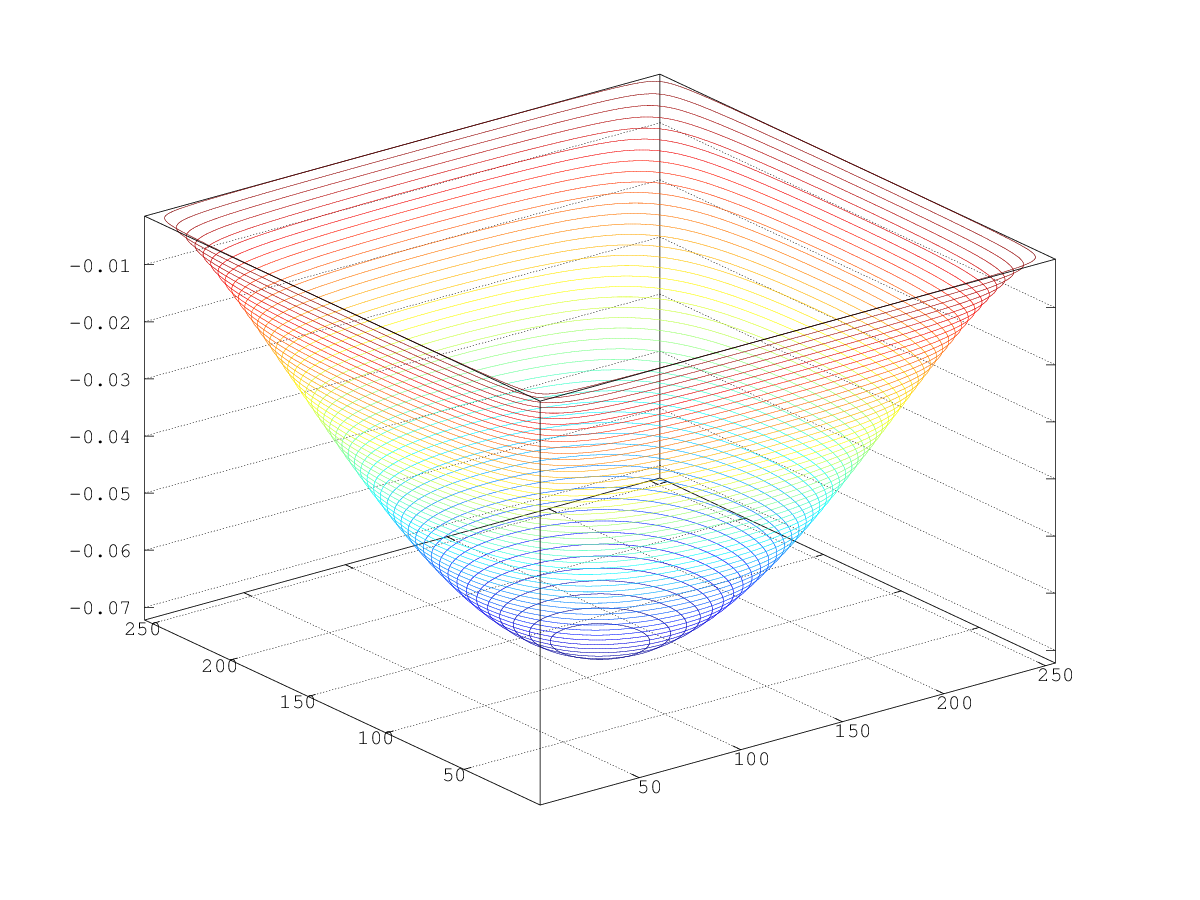
\includegraphics[width=0.7\textwidth]{datashit512flat_v2.png}
    \caption{$H^2$}
\end{figure}

\begin{figure}[t]
  \centering
    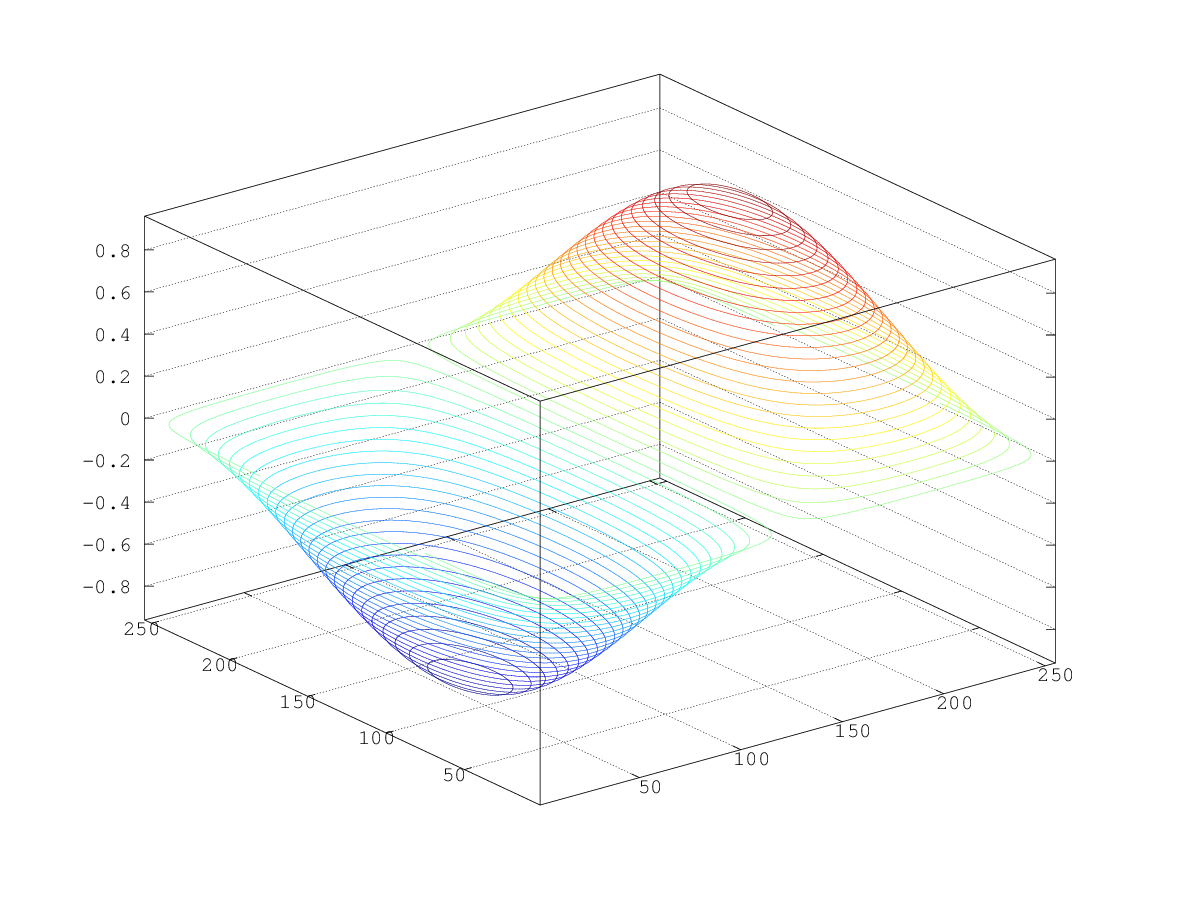
\includegraphics[width=0.7\textwidth]{datashit512sinpixsin2pix_v2.png}
    \caption{$(sin(\pi*x)\cdot sin(2\pi*y))\cdot 5\pi^2$}
\end{figure}
\FloatBarrier
We did some testing with various problem sizes to see how fast our program ran, then we
extrapolated the expected run time by using:
\begin{align}
k &= 
    \dfrac{n_{0}^2*\log{n_{0}}}{t}
\end{align}
\begin{align}    
t_{n} &= \dfrac
        {n^2\cdot\log{n}}
        {k} 
\end{align}

\begin{figure}[t]
  \centering
    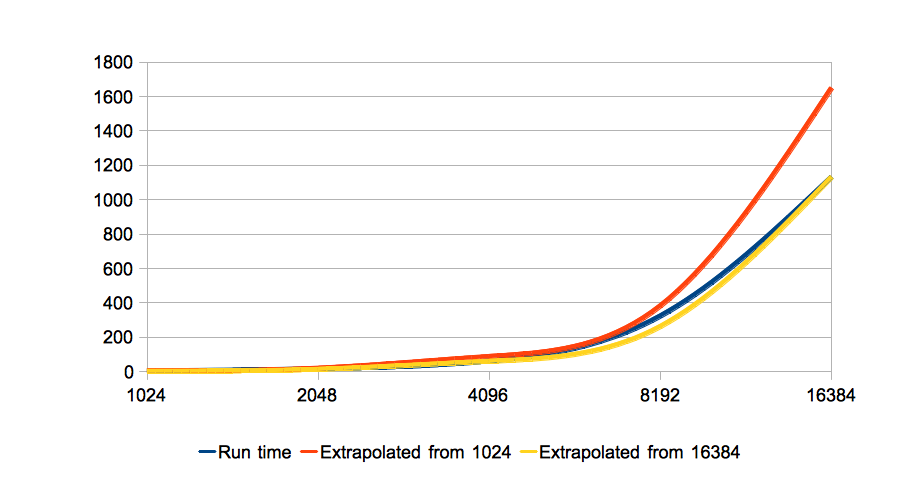
\includegraphics[width=0.8\textwidth]{speed_over_size_3.png}
    \caption{Run time for various problem sizes, compared to their extrapolation}
    \label{runsize}
\end{figure}

To show a $n^2\cdot$log n extrapolation from the actual run time, as shown in figure \ref{runsize}, where we did an extrapolation from the run time of a problem set of size 1024 and up, and a similar extrapolation from the run time of a problem set of size 16 384. This shows that our runtime scales within the expected values, although the extrapolation looks closer when basing it on 16 384 than when basing it on 1024. This is partially because the smaller problem sets fit better into cache, but also because the actual run time dominates less than the constant-factors at these sizes.

We also did a comparison with regards to how our program scales with the amount of processes it is run with,
as shown in figure \ref{numprocs}, our run time does indeed go down, with an odd increase in speed between 6 processes and 9 processes.
\begin{figure}[t]
  \centering
    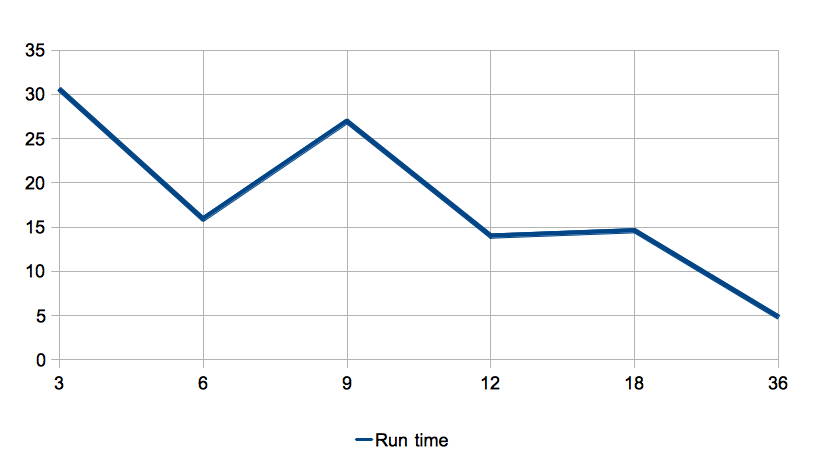
\includegraphics[width=0.8\textwidth]{run_time_over_np.png}
    \caption{Run time for problem size 4096 with varying process-amount}
    \label{numprocs}
\end{figure}

\FloatBarrier